\documentclass[aspectratio=1610]{beamer}
\usepackage[T1]{fontenc}
\usetheme{wildcat}

\usepackage{amsmath,amssymb,amsfonts}
%\usepackage{booktabs}
\usepackage{relsize}
\usepackage[export]{adjustbox}
\usepackage{environ}
\usepackage{fancyvrb} 
\usepackage{listings}
\lstset{%
  basicstyle=\small\ttfamily\color{wcprimary},
  language=[LaTeX]{TeX},
  backgroundcolor=\color{white},
  xleftmargin=0.1cm,
  rulecolor=\color{wcprimary},
  frame=single,
  aboveskip=7pt,
  %framesep=8pt,
  %framerule=1pt
}

\usepackage[style=verbose,backend=biber]{biblatex}
\addbibresource{references.bib}
\let\oldfootnotesize\footnotesize
\renewcommand*{\footnotesize}{\oldfootnotesize\tiny}

\def\mathdefault#1{#1}
\everymath=\expandafter{\the\everymath\displaystyle}

% Define a new environment 'splitframe'
\NewEnviron{splitframe}[1]{%
  \begin{frame}[fragile]{#1}
    \begin{columns}[T]
      % Left column: Display S(L) using fancyvrb’s Verbatim.
      \column{0.50\textwidth}
        \begin{Verbatim}
\BODY
        \end{Verbatim}
      % Right column: Execute L.
      \column{0.50\textwidth}
\BODY
    \end{columns}
  \end{frame}
}


\title{\LaTeX{} 101 \\ {\small ME 800 Seminar}}
\date{April 15, 2025}
\author{Jeremy Roberts}

\begin{document}

\begin{frame}
  \titlepage
\end{frame}

\section{Standalone \LaTeX{} Documents}

%%%%%%%%%%%%%%%%%%%%%%%%%%%%%%%%%%%%%%%%%%%%%%%%%%%%%%%%%%%%%%%%%%%%%%%%%%%%%%%
\begin{frame}[fragile]{A Barebones Document}
  \begin{columns}[T]

    \column{0.50\textwidth}

      \lstinputlisting[]{example_article.tex}

      \vspace{0.25cm}

      \raggedleft {\it Shown above is the \textcolor{wcprimary}{plain-text, LaTeX source}.  At right is
      the compiled PDF, and below, a zoomed view of the PDF.}

      \vspace{0.25cm}

      
\includegraphics[width=1.01\textwidth, trim={5cm 22cm 8cm 3cm},
                       clip, frame]{example_article.pdf}


    \column{0.50\textwidth}
      %  trim={<left> <lower> <right> <upper>}

      
\includegraphics[width=0.9\textwidth, frame]{example_article.pdf}

  \end{columns}
\end{frame}

%%%%%%%%%%%%%%%%%%%%%%%%%%%%%%%%%%%%%%%%%%%%%%%%%%%%%%%%%%%%%%%%%%%%%%%%%%%%%%%
\begin{frame}[fragile]{The Preamble and some {\it Lorem Ipsum}}
  \begin{columns}[T]

    \column{0.50\textwidth}

      \lstinputlisting{example_lorem.tex}

      \raggedleft {\small\it The default fonts come from the Computer Modern family invented by
      Donald Knuth, who also invented the low-level, great-for-math 
      typesetting language \TeX{}.}

    \column{0.50\textwidth}
      %  trim={<left> <lower> <right> <upper>}

      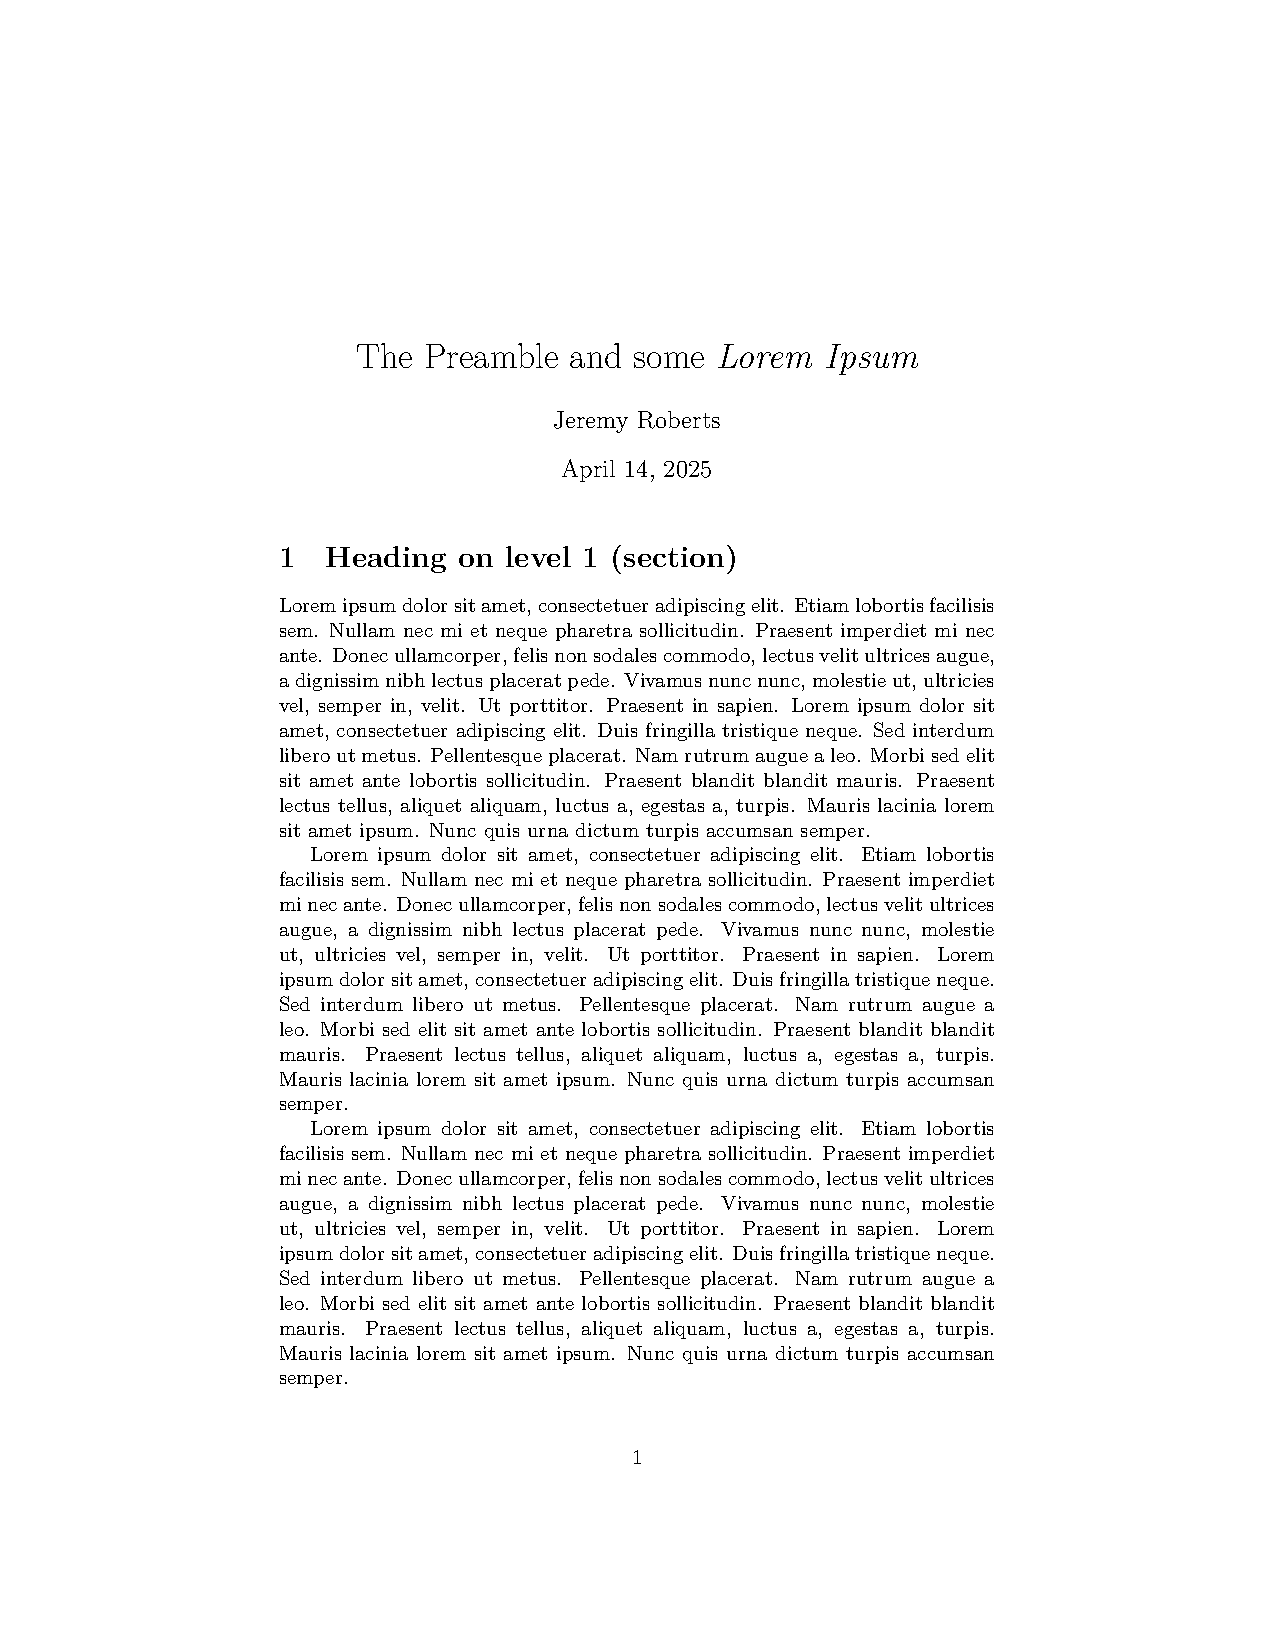
\includegraphics[width=0.9\textwidth, frame]{example_lorem.pdf}

  \end{columns}
\end{frame}


%%%%%%%%%%%%%%%%%%%%%%%%%%%%%%%%%%%%%%%%%%%%%%%%%%%%%%%%%%%%%%%%%%%%%%%%%%%%%%%
\begin{frame}[fragile]{Tweaking Formats}
  \begin{columns}[T]

    \column{0.50\textwidth}

      \lstinputlisting{example_formatting.tex}
      \raggedleft {\small\it \LaTeX{} is a higher-level markup language 
      built on \TeX{} that simplifies document preparation by providing structured commands and environments for formatting.}

    \column{0.50\textwidth}
      %  trim={<left> <lower> <right> <upper>}

      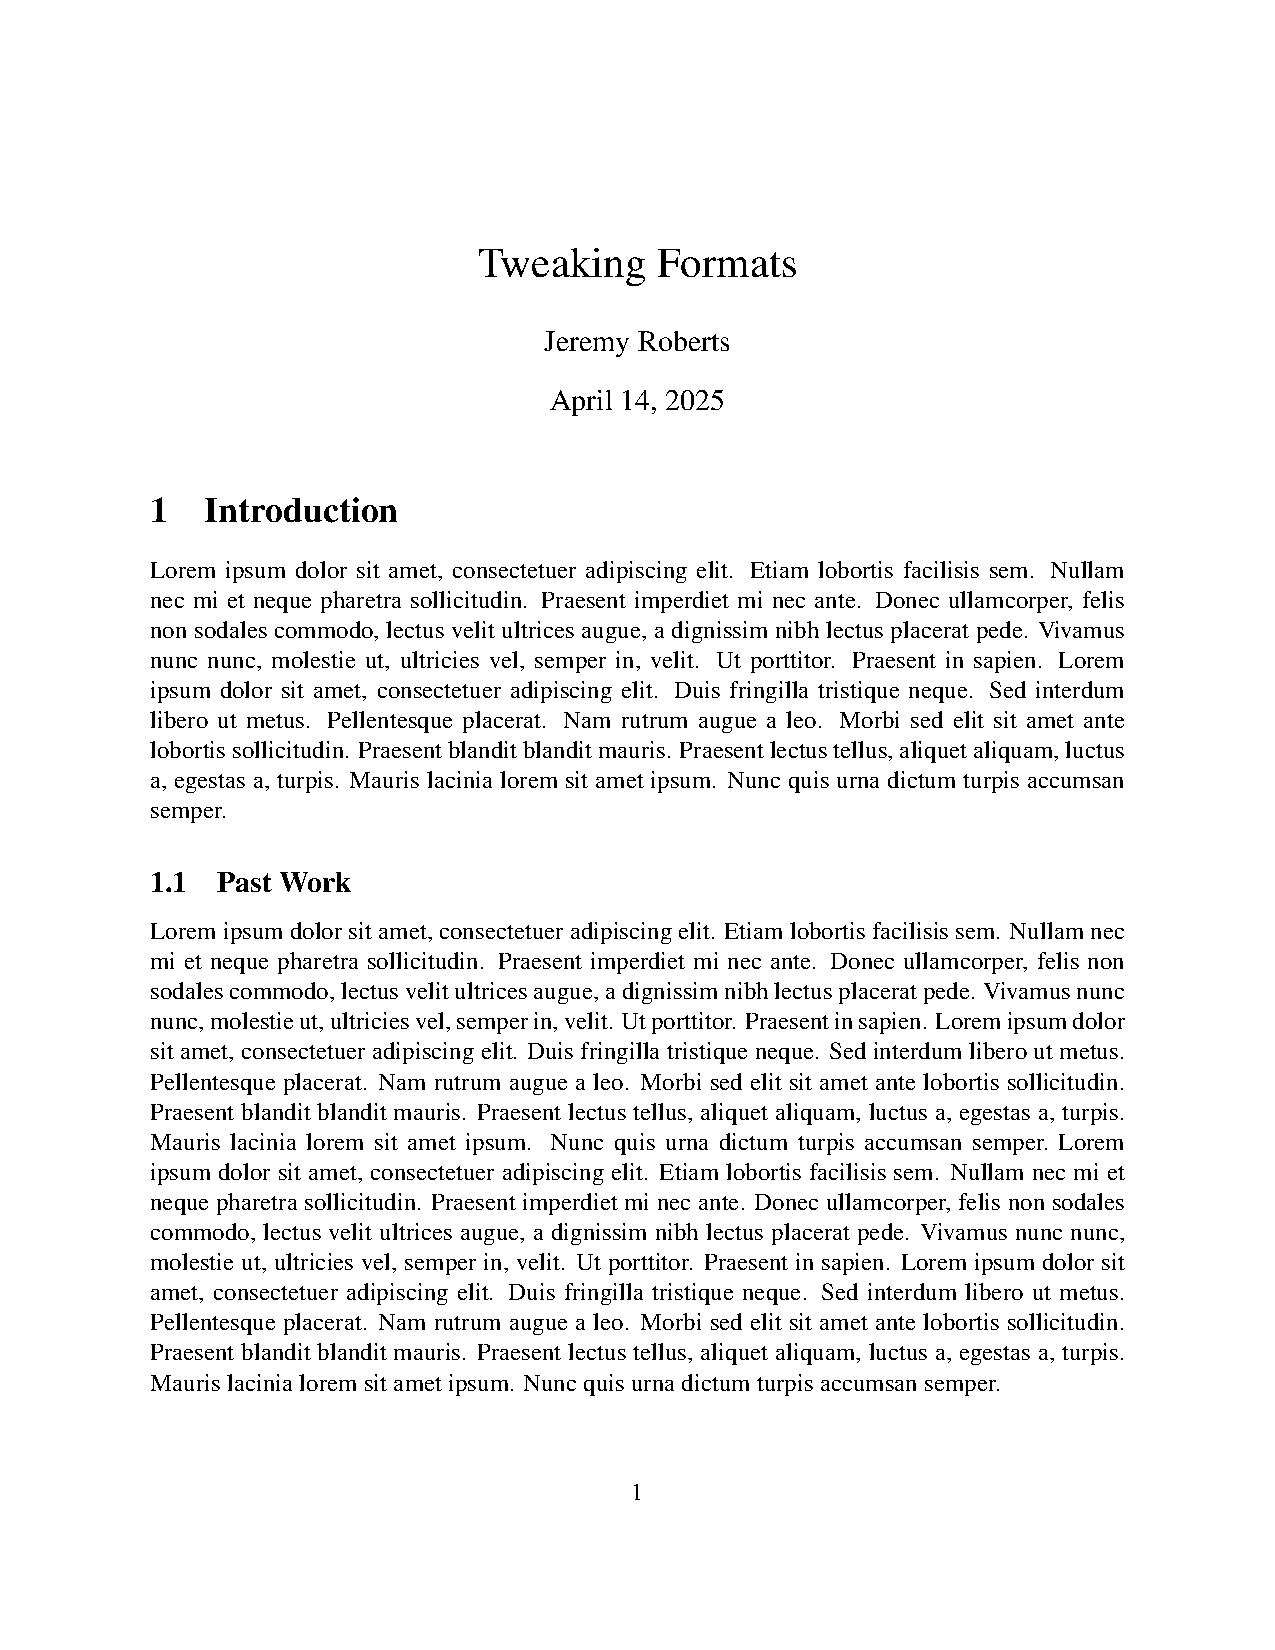
\includegraphics[width=0.9\textwidth, frame]{example_formatting.pdf}

  \end{columns}
\end{frame}

%%%%%%%%%%%%%%%%%%%%%%%%%%%%%%%%%%%%%%%%%%%%%%%%%%%%%%%%%%%%%%%%%%%%%%%%%%%%%%%
\begin{frame}[fragile]{A Journal Article}
  \begin{columns}[T]

    \column{0.50\textwidth}

      \vspace{-5pt}

      \lstinputlisting[basicstyle=\footnotesize\ttfamily\color{wcprimary}]{example_journal.tex}

      \raggedleft {\it Many templates and classes available!}

    \column{0.50\textwidth}

      %  trim={<left> <lower> <right> <upper>}
      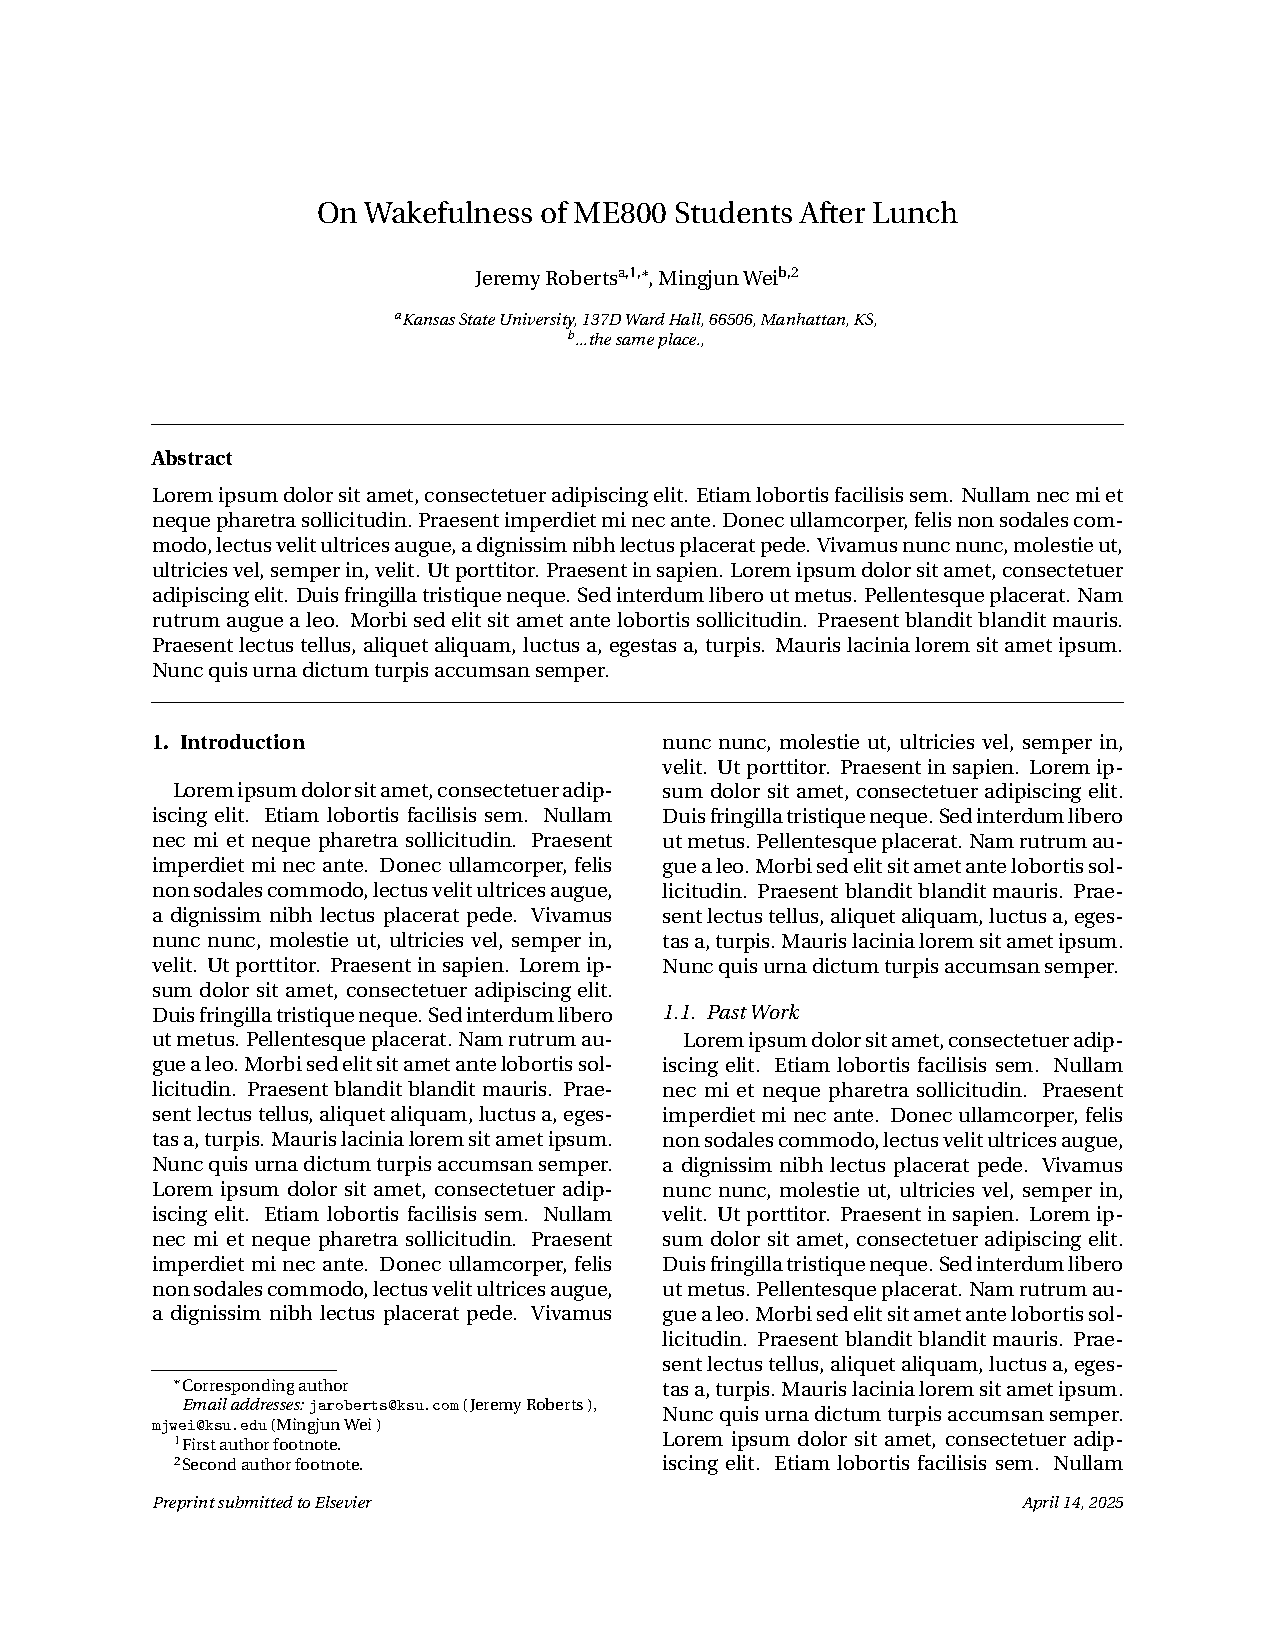
\includegraphics[width=0.9\textwidth, frame]{example_journal.pdf}

  \end{columns}
\end{frame}

%%%%%%%%%%%%%%%%%%%%%%%%%%%%%%%%%%%%%%%%%%%%%%%%%%%%%%%%%%%%%%%%%%%%%%%%%%%%%%%
\begin{frame}[fragile]{Thesis Support}

  \begin{columns}[T]

    \column{0.55\textwidth}

      \begin{itemize}
      \item An official \LaTeX{} template is available for K-State theses and dissertations:\\
          \url{https://www.k-state.edu/grad/academics/etdr/template/}
      \item A video tutorial is available:\\
          \url{https://youtu.be/XyiD893gpR4}
      \item The template is also available on Overleaf!
      \end{itemize}

    \column{0.45\textwidth}

      
\includegraphics[width=0.99\textwidth, frame]{example_thesis.pdf}

  \end{columns}

\end{frame}


%%%%%%%%%%%%%%%%%%%%%%%%%%%%%%%%%%%%%%%%%%%%%%%%%%%%%%%%%%%%%%%%%%%%%%%%%%%%%%%
\section{Core \LaTeX{} Structures}

%%%%%%%%%%%%%%%%%%%%%%%%%%%%%%%%%%%%%%%%%%%%%%%%%%%%%%%%%%%%%%%%%%%%%%%%%%%%%%%
\begin{frame}[fragile]{Lists and Enumerations}
  \begin{columns}[T]

    \column{0.50\textwidth}

\begin{lstlisting}
Unumbered lists of items:
\begin{itemize}
   \item First level item
   \item First level item
   \begin{itemize}
     \item Second level item
     \item Second level item
   \end{itemize}
\end{itemize}

Numbered lists:
\begin{enumerate}
    \item Item one
    \item Item two
\end{enumerate}
\end{lstlisting}

    \column{0.50\textwidth}

 \vbox to .7\textheight{%
 
Unumbered lists of items:
\begin{itemize}
   \item First level item 1
   \item First level item 2
   
   \begin{itemize}
     \item Second level item 1
     \item Second level item 2
   \end{itemize}
\end{itemize}


Numbered lists:
\begin{enumerate}
    \item Item 1
    \item Item 2
\end{enumerate}



\raggedleft {\it Like with code, it helps
to use white space to improve readability
of \LaTeX{}.}
}
  \end{columns}

\end{frame}

%%%%%%%%%%%%%%%%%%%%%%%%%%%%%%%%%%%%%%%%%%%%%%%%%%%%%%%%%%%%%%%%%%%%%%%%%%%%%%%
\begin{frame}[fragile]{Basic Equations}
  \begin{columns}[T]
    % Left column: S(L)
    \column{0.50\textwidth}
      \begin{lstlisting}
Inline math is writing an 
equation like $E=mc^2$ as 
part of a sentence, while 
we can offset math by
\[
  I = \int_a^b f(x) dx \, .
\]
Equations can be numbered like
\begin{equation}
 E = mc^2  
 \label{eq:einstein}
\end{equation}
and referenced as 
Eq.~(\ref{eq:einstein}). They
can also be unnumbered, like
\begin{equation*}
  I = \int_a^b f(x) dx \, .
\end{equation*}
      \end{lstlisting}
    % Right column: L (the block executed)
    \column{0.50\textwidth}
%%%%%%%%%%%%%%%%%%%%%%%%%%%%%%%%%%%%%%%
Inline math is writing an 
equation like $E=mc^2$ as 
part of a sentence, while 
we can offset math by
\[
  I = \int_a^b f(x) dx \, .
\]
Equations can be numbered like
\begin{equation}
 E = mc^2  
 \label{eq:einstein}
\end{equation}
and referenced as 
Eq.~(\ref{eq:einstein}). They
can also be unnumbered, like
\begin{equation*}
  I = \int_a^b f(x) dx \, .
\end{equation*}
%%%%%%%%%%%%%%%%%%%%%%%%%%%%%%%%%%%%%%%%%%%
  \end{columns}
\end{frame}

%%%%%%%%%%%%%%%%%%%%%%%%%%%%%%%%%%%%%%%%%%%%%%%%%%%%%%%%%%%%%%%%%%%%%%%%%%%%%%%
\begin{frame}[fragile]{Mathematical Symbols}
  \begin{columns}[T]
    % Left column: S(L)
    \column{0.50\textwidth}
      \begin{lstlisting}[basicstyle=\footnotesize\ttfamily\color{wcprimary}]
Many mathematical symbols are made available 
by using the {\tt amsmath} package:
\begin{math}
\begin{array}{ccccc}
\alpha  & \beta   & \pi       & \Phi      & \zeta   \\
\sum    & \prod   & \int      & \partial  & \nabla  \\
\vec{x} & \hat{x} & \dot{x}   & \tilde{x} & \bar{x} \\
\in     & \notin  & \subset   & \subseteq & \cup    \\
\leq    & \geq    & \approx   & \equiv    & \neq    \\
\forall & \exists & \emptyset & \infty    & \angle  \\
\mathrm{X} & \mathbf{X} & \mathbb{X} & \mathcal{X} 
& \mathfrak{X} \\ 
\boldsymbol{\pi} & & & & \\  
\end{array}
\end{math}

      \end{lstlisting}
    % Right column: L (the block executed)
    \column{0.50\textwidth}
%%%%%%%%%%%%%%%%%%%%%%%%%%%%%%%%%%%%%%%
\begin{math}
\begin{array}{ccccc}
\alpha  & \beta   & \pi       & \Phi      & \zeta   \\
\sum    & \prod   & \int      & \partial  & \nabla  \\
\vec{x} & \hat{x} & \dot{x}   & \tilde{x} & \bar{x} \\
\in     & \notin  & \subset   & \subseteq & \cup    \\
\leq    & \geq    & \approx   & \equiv    & \neq    \\
\forall & \exists & \emptyset & \infty    & \angle  \\
\mathrm{X} & \mathbf{X} & \mathbb{X} & \mathcal{X} 
& \mathfrak{X} \\ 
\boldsymbol{\pi} & & & & \\  
\end{array}
\end{math}
%%%%%%%%%%%%%%%%%%%%%%%%%%%%%%%%%%%%%%%%%%%
  \end{columns}
\end{frame}

%%%%%%%%%%%%%%%%%%%%%%%%%%%%%%%%%%%%%%%%%%%%%%%%%%%%%%%%%%%%%%%%%%%%%%%%%%%%%%%
\begin{frame}[fragile]{Aligned Equations}
  \begin{columns}[T]
% Left column: S(L)
    \column{0.50\textwidth}
      \begin{lstlisting}
Equations sometimes require
multiple lines like
\begin{equation}
 \begin{split}
  (a+1)x + by &= c \\
      dx + ey &= f \, ,
 \end{split}
\end{equation}
where the {\tt \&=} horizontally 
aligns the equations at the $=$ 
symbol.  Equivalently,
\begin{align}
  (a+1)x + by &= c \\
      dx + ey &= f \, .
\end{align}
      \end{lstlisting}
    \column{0.50\textwidth}
%%%%%%%%%%%%%%%%%%%%%%%%%%%%%%%%%%%%%%%%%%%
Equations sometimes require
multiple lines like
\begin{equation}
 \begin{split}
  (a+1)x + by &= c \\
      dx + ey &= f \, ,
 \end{split}
\end{equation}
where the {\tt \&=} horizontally 
aligns the equations at the $=$ 
symbol.  Equivalently,
\begin{align}
  (a+1)x + by &= c \\
      dx + ey &= f \, .
\end{align}
%%%%%%%%%%%%%%%%%%%%%%%%%%%%%%%%%%%%%%%%%%%
\raggedleft {\it Align equations in 
the \LaTeX{} source for easier revisions.}
  \end{columns}
\end{frame}

%%%%%%%%%%%%%%%%%%%%%%%%%%%%%%%%%%%%%%%%%%%%%%%%%%%%%%%%%%%%%%%%%%%%%%%%%%%%%%%
\begin{frame}[fragile]{Tables and Figures}
  \begin{columns}[T]
    \column{0.50\textwidth}
      \begin{lstlisting}
\begin{table}[h]
  \centering
  \begin{tabular}{lcr}
    \toprule
    Item   & Price  & Quantity \\
    \midrule
    Apple  & \$1.00 & 10       \\
    Banana & \$0.50 & 20       \\
    \bottomrule
  \end{tabular}
  \caption{Fruit Prices}
\end{table}

\begin{figure}[h]
  \centering
  \fbox{Sample Figure}
  \caption{Sample Figure}
\end{figure}
      \end{lstlisting}
    \column{0.50\textwidth}
\begin{table}[h]
  \centering
  \begin{tabular}{lcr}
    %\toprule
    Item   & Price  & Quantity \\
   % \midrule
    Apple  & \$1.00 & 10       \\
    Banana & \$0.50 & 20       \\
  %  \bottomrule
  \end{tabular}
  \caption{Fruit Prices}
\end{table}

\begin{figure}[h]
  \centering
  \fbox{Sample Figure}
  \caption{Sample Figure}
\end{figure}
  \end{columns}
\end{frame}

%%%%%%%%%%%%%%%%%%%%%%%%%%%%%%%%%%%%%%%%%%%%%%%%%%%%%%%%%%%%%%%%%%%%%%%%%%%%%%%
% \begin{frame}[fragile]{Bibliography and References}
%   \begin{columns}[T]
%     \column{0.50\textwidth}
%       \begin{lstlisting}
% See \cite{lamport1994latex} for LaTeX basics.
% 
% \section{Introduction}\label{sec:intro}
% 
% Refer to Section~\ref{sec:intro} for more details.
% 
% \printbibliography
%       \end{lstlisting}
%     \column{0.50\textwidth}
% See \cite{lamport1994latex} for LaTeX basics.
% 
% \section{Introduction}\label{sec:intro}
% 
% Refer to Section~\ref{sec:intro} for more details.
% 
% \printbibliography
%   \end{columns}
% \end{frame}



%%%%%%%%%%%%%%%%%%%%%%%%%%%%%%%%%%%%%%%%%%%%%%%%%%%%%%%%%%%%%%%%%%%%%%%%%%%%%%%
\begin{frame}[fragile]{Matrices}
  \begin{columns}[T]
    \column{0.50\textwidth}
      \begin{lstlisting}
Matrices have many forms:
\begin{align*}
 \begin{array}{cc} a & b\\ c & d 
   \end{array} & \quad
 \begin{smallmatrix}a & b\\ c & d 
   \end{smallmatrix} \\
  & \begin{matrix} a & b \\ c & d 
   \end{matrix} \quad 
 \begin{bmatrix} a & b \\ c & d 
   \end{bmatrix} & \\
 \begin{pmatrix} a & b \\ c & d 
   \end{pmatrix} & \quad
 \begin{Bmatrix} a & b \\ c & d 
   \end{Bmatrix} \\
 \begin{vmatrix} a & b \\ c & d 
   \end{vmatrix} \quad 
 \begin{Vmatrix} a & b \\ c & d 
   \end{Vmatrix} & \\
\end{align*}
      \end{lstlisting}
    \column{0.50\textwidth}
Matrices have many forms:
\begin{align*}
 \begin{array}{cc} a & b\\ c & d 
   \end{array} & \quad
 \begin{smallmatrix}a & b\\ c & d 
   \end{smallmatrix} \\
  & \begin{matrix} a & b \\ c & d 
   \end{matrix} \quad 
 \begin{bmatrix} a & b \\ c & d 
   \end{bmatrix} & \\
 \begin{pmatrix} a & b \\ c & d 
   \end{pmatrix} & \quad
 \begin{Bmatrix} a & b \\ c & d 
   \end{Bmatrix} \\
 \begin{vmatrix} a & b \\ c & d 
   \end{vmatrix} \quad 
 \begin{Vmatrix} a & b \\ c & d 
   \end{Vmatrix} & \\
\end{align*}
  \end{columns}
\end{frame}

% \[
% f(x)=
% \begin{cases}
% x^2,   & \text{if } x \ge 0, \\
% -x^2,  & \text{if } x < 0.
% \end{cases}
% \]

%%%%%%%%%%%%%%%%%%%%%%%%%%%%%%%%%%%%%%%%%%%%%%%%%%%%%%%%%%%%%%%%%%%%%%%%%%%%%%%
\begin{frame}[fragile]{LaTeX in Jupyter}
  \begin{columns}[T]
    \column{0.50\textwidth}
      \begin{lstlisting}
% Examples of platforms supporting LaTeX rendering:
- Jupyter Notebook: Markdown cells support inline math ($...$)
  and display math ($$...$$) via MathJax.
- Overleaf: Online LaTeX editor with live preview.
- GitHub: README files and issues support LaTeX via MathJax.
- StackExchange: Sites like Math.SE support LaTeX.
      \end{lstlisting}
    \column{0.50\textwidth}
% Examples of platforms supporting LaTeX rendering:
- Jupyter Notebook: Markdown cells support inline math ($...$)
  and display math ($$...$$) via MathJax.
- Overleaf: Online LaTeX editor with live preview.
- GitHub: README files and issues support LaTeX via MathJax.
- StackExchange: Sites like Math.SE support LaTeX.
  \end{columns}
\end{frame}

%%%%%%%%%%%%%%%%%%%%%%%%%%%%%%%%%%%%%%%%%%%%%%%%%%%%%%%%%%%%%%%%%%%%%%%%%%%%%%%
\begin{frame}[fragile]{LaTeX in Word and Canvas Equations}
  \begin{columns}[T]
    \column{0.50\textwidth}
      \begin{lstlisting}
% Examples of platforms with LaTeX-like equation support:
- Microsoft Word: Equation Editor supports LaTeX-like syntax.
- Canvas LMS: Math input fields accept LaTeX-style code.
- Google Docs: With add-ons for LaTeX equations.
- LibreOffice: The Math component supports similar syntax.
      \end{lstlisting}
    \column{0.50\textwidth}
% Examples of platforms with LaTeX-like equation support:
- Microsoft Word: Equation Editor supports LaTeX-like syntax.
- Canvas LMS: Math input fields accept LaTeX-style code.
- Google Docs: With add-ons for LaTeX equations.
- LibreOffice: The Math component supports similar syntax.
  \end{columns}
\end{frame}

% %%%%%%%%%%%%%%%%%%%%%%%%%%%%%%%%%%%%%%%%%%%%%%%%%%%%%%%%%%%%%%%%%%%%%%%%%%%%%%%
% \begin{frame}[fragile]{Beamer Presentations}
%   \begin{columns}[T]
%     \column{0.50\textwidth}
%       \begin{lstlisting}
% \begin{frame}{Sample Slide}
% This is a sample slide created with Beamer.
% \end{frame}
%       \end{lstlisting}
%     \column{0.50\textwidth}
%       % Since nesting a frame inside a frame is problematic,
%       % we simulate the output with a minipage.
%       \begin{minipage}{\linewidth}
%         \centering
%         {\bf Sample Slide}\\[1ex]
%         This is a sample slide created with Beamer.
%       \end{minipage}
%   \end{columns}
% \end{frame}

% %%%%%%%%%%%%%%%%%%%%%%%%%%%%%%%%%%%%%%%%%%%%%%%%%%%%%%%%%%%%%%%%%%%%%%%%%%%%%%%
% \begin{frame}[fragile]{Conference Posters with LaTeX}
%   \begin{columns}[T]
%     \column{0.50\textwidth}
%       \begin{lstlisting}
% \title{Sample Poster Title}
% \author{Jane Doe}
% \maketitle
% \block{Introduction}{
% This is the introduction section of the poster.
% }
%       \end{lstlisting}
%     \column{0.50\textwidth}
%       % Simulated output using standard text and a block.
%       \begin{minipage}{\linewidth}
%         \centering
%         {\Large Sample Poster Title}\\[1ex]
%         {\large Jane Doe}\\[1ex]
%         \par\medskip
%         \textbf{Introduction}\\[0.5ex]
%         This is the introduction section of the poster.
%       \end{minipage}
%   \end{columns}
% \end{frame}

%%%%%%%%%%%%%%%%%%%%%%%%%%%%%%%%%%%%%%%%%%%%%%%%%%%%%%%%%%%%%%%%%%%%%%%%%%%%%%%
\begin{frame}
  \centering
  \Huge Questions?
\end{frame}

% https://www.texifier.com/docs/tutorials/tex/advanced/tex-vs-latex

\end{document}

